\subsection{UDP / TCP}
To analyze the difference in power consumption between the two transmission methods,
we compare them. In the analysis we pay attention to the elapsed time and the power consumption while the
ESP8266 transmits. In the first comparsion, we compare 100 trasmitting cicles.
\linebreak
\begin{table}[H]
    \begin{center}
    \caption{Comparison TCP UDP}
    \label{tab:table3}
    \renewcommand{\arraystretch}{1.8}
    \begin{tabular}{l|c|c|r}
    & \textbf{TCP} & \textbf{UDP} & \textbf{difference} \\
    & \multicolumn{2}{c|}{elapsed time [ms]} & \textbf{\%}\\
    \hline
    count & 100 & 100 & \\
    mean  & 241.57 & 95.97 & 39.73 \\
    std   & 32.115403 & 1.058444 & 3.30 \\
    min   & 193.0 & 94.0 & 48.70 \\
    25\%  & 219.0 & 95.0 & 43.38 \\
    50\%  & 236.0 & 96.0 & 40.68 \\
    75\%  & 257.0 & 97.0 & 37.74 \\
    max   & 396.0 & 98.0 & 24.75 \\
    \end{tabular}
    \end{center}
\end{table}
\begin{figure}[H]
    \centering
    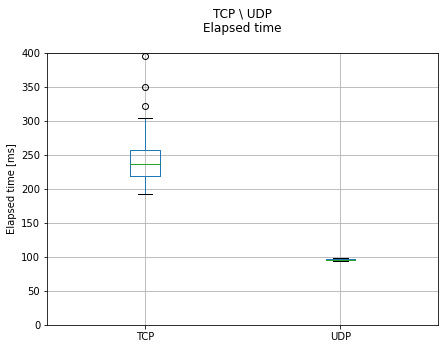
\includegraphics[width = 0.9 \linewidth]{fig/udp_tcp/udp_tcp_boxplot_time.png}
    \caption{Elapsed time when sending data over TCP and UDP}
    \label{fig:udp_tcp_boxplot_time}
    \end{figure}
If we compare the elapsed time spent sending the 1000 bytes,
we can save 96.0048$\pm$11.145 ms for a send cycle.
As shown in Table\ref{tab:table3},
we see that the range between the maximum and minimum send time for UDP is also much smaller.
As described in Chapter \ref{udp:sci}, UDP has less overhead when sending.
That's why it doesn't need energy to monitor sending cycle.
\begin{table}[H]
    \begin{center}
    \caption{Comparison TCP UDP}
    \label{tab:table4}
    \renewcommand{\arraystretch}{1.8}
    \begin{tabular}{l|c|c|r}
    & \textbf{TCP} & \textbf{{UDP}} & \textbf{difference} \\
    & \multicolumn{2}{c|}{ power consumption [As]} & \textbf{\%}\\
    \hline
    count & 100 & 100 & \\
    mean   & 0.021031 & 0.009227 & 43.87 \\
    std    & 0.002591 & 0.000581 & 22.42 \\
    min    & 0.0163 & 0.0082 & 50.31 \\
    25\%   & 0.019175 & 0.0088 & 45.89 \\
    50\%   & 0.0206 & 0.0091 & 44.17 \\
    75\%   & 0.022325 & 0.0096 & 43.00 \\
    max    & 0.0326 & 0.0109 & 33.44 \\
    \end{tabular}
    \end{center}
\end{table}
\begin{figure}[H]
    \centering
    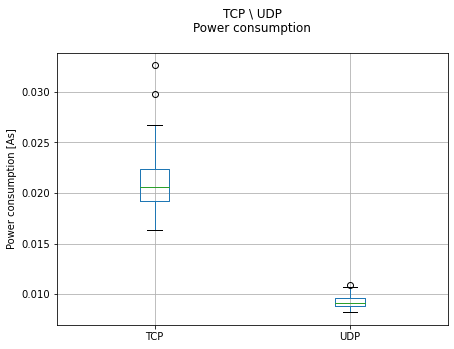
\includegraphics[width = 0.9 \linewidth]{fig/udp_tcp/udp_tcp_boxplot_As.png}
    \caption{Power connsumption when sending data over TCP and UDP}
    \label{fig:udp_tcp_boxplot_As}
    \end{figure}
In Table\ref{tab:table4} we compared the elapsed time while the ESP8266 sends.
As expected, we get the same result.
UDP requires only 44.03\%$\pm$6.07\% of the time compared to TCP.
This gives us a saving of 0.00907018$\pm$0.00125 As while sending 1000 bytes.
For example, in Fig.\ref{fig:udp_tcp_s_m},
we compare the iteration 50 to see the differences between the two.
The power consumption of UDP increases the first time the connection
is started and the second part is exactly when it sends.
In contrast, TCP requires much more power to establish the connection and waits before sending.
\begin{figure}[H]
    \centering
    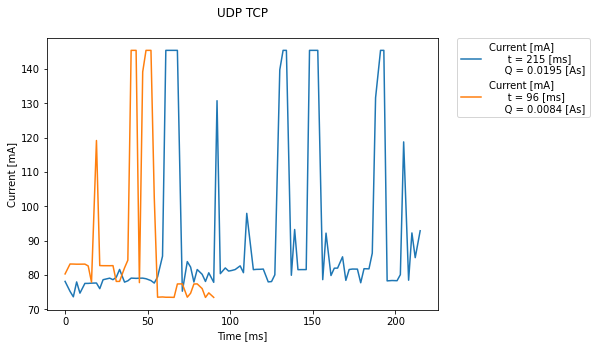
\includegraphics[width = 1 \linewidth]{fig/udp_tcp/udp_tcp_s_m.png}
    \caption{Sending data over TCP and UDP}
    \label{fig:udp_tcp_s_m}
    \end{figure}